%
%Не забыть:
%--------------------------------------
%Вставить колонтитулы, поменять название на титульнике



%--------------------------------------

\documentclass[a4paper, 12pt]{article} 

%--------------------------------------
%Russian-specific packages
%--------------------------------------
%\usepackage[warn]{mathtext}
\usepackage[T2A]{fontenc}
\usepackage[utf8]{inputenc}
\usepackage[english,russian]{babel}
\usepackage[intlimits]{amsmath}
\usepackage{esint}
%--------------------------------------
%Hyphenation rules
%--------------------------------------
\usepackage{hyphenat}
\hyphenation{ма-те-ма-ти-ка вос-ста-нав-ли-вать}
%--------------------------------------
%Packages
%--------------------------------------
\usepackage{amsmath}
\usepackage{amssymb}
\usepackage{amsfonts}
\usepackage{amsthm}
\usepackage{latexsym}
\usepackage{mathtools}
\usepackage{etoolbox}%Булевые операторы
\usepackage{extsizes}%Выставление произвольного шрифта в \documentclass
\usepackage{geometry}%Разметка листа
\usepackage{indentfirst}
\usepackage{wrapfig}%Создание обтекаемых текстом объектов
\usepackage{fancyhdr}%Создание колонтитулов
\usepackage{setspace}%Настройка интерлиньяжа
\usepackage{lastpage}%Вывод номера последней страницы в документе, \lastpage
\usepackage{soul}%Изменение параметров начертания
\usepackage{hyperref}%Две строчки с настройкой гиперссылок внутри получаеммого
\usepackage[usenames,dvipsnames,svgnames,table,rgb]{xcolor}% pdf-документа
\usepackage{multicol}%Позволяет писать текст в несколько колонок
\usepackage{cite}%Работа с библиографией
\usepackage{subfigure}% Человеческая вставка нескольких картинок
\usepackage{tikz}%Рисование рисунков
\usepackage{float}% Возможность ставить H в положениях картинки
% Для картинок Моти
\usepackage{misccorr}
\usepackage{lscape}
\usepackage{cmap}



\usepackage{graphicx,xcolor}
\graphicspath{{Pictures/}}
\DeclareGraphicsExtensions{.pdf,.png,.jpg}

%----------------------------------------
%Список окружений
%----------------------------------------
\newenvironment {theor}[2]
{\smallskip \par \textbf{#1.} \textit{#2}  \par $\blacktriangleleft$}
{\flushright{$\blacktriangleright$} \medskip \par} %лемма/теорема с доказательством
\newenvironment {proofn}
{\par $\blacktriangleleft$}
{$\blacktriangleright$ \par} %доказательство
%----------------------------------------
%Список команд
%----------------------------------------
\newcommand{\grad}
{\mathop{\mathrm{grad}}\nolimits\,} %градиент

\newcommand{\diver}
{\mathop{\mathrm{div}}\nolimits\,} %дивергенция

\newcommand{\rot}
{\ensuremath{\mathrm{rot}}\,}

\newcommand{\Def}[1]
{\underline{\textbf{#1}}} %определение

\newcommand{\RN}[1]
{\MakeUppercase{\romannumeral #1}} %римские цифры

\newcommand {\theornp}[2]
{\textbf{#1.} \textit{ #2} \par} %Написание леммы/теоремы без доказательства

\newcommand{\qrq}
{\ensuremath{\quad \Rightarrow \quad}} %Человеческий знак следствия

\newcommand{\qlrq}
{\ensuremath{\quad \Leftrightarrow \quad}} %Человеческий знак равносильности

\renewcommand{\phi}{\varphi} %Нормальный знак фи

\newcommand{\me}
{\ensuremath{\mathbb{E}}}

\newcommand{\md}
{\ensuremath{\mathbb{D}}}



%\renewcommand{\vec}{\overline}




%----------------------------------------
%Разметка листа
%----------------------------------------
\geometry{top = 3cm}
\geometry{bottom = 2cm}
\geometry{left = 1.5cm}
\geometry{right = 1.5cm}
%----------------------------------------
%Колонтитулы
%----------------------------------------
\pagestyle{fancy}%Создание колонтитулов
\fancyhead{}
%\fancyfoot{}
%\fancyhead[R]{\textsc{Получение и измерение вакуума}}%Вставить колонтитул сюда
%----------------------------------------
%Интерлиньяж (расстояния между строчками)
%----------------------------------------
%\onehalfspacing -- интерлиньяж 1.5
%\doublespacing -- интерлиньяж 2
%----------------------------------------
%Настройка гиперссылок
%----------------------------------------
\hypersetup{				% Гиперссылки
	unicode=true,           % русские буквы в раздела PDF
	pdftitle={Заголовок},   % Заголовок
	pdfauthor={Автор},      % Автор
	pdfsubject={Тема},      % Тема
	pdfcreator={Создатель}, % Создатель
	pdfproducer={Производитель}, % Производитель
	pdfkeywords={keyword1} {key2} {key3}, % Ключевые слова
	colorlinks=true,       	% false: ссылки в рамках; true: цветные ссылки
	linkcolor=blue,          % внутренние ссылки
	citecolor=blue,        % на библиографию
	filecolor=magenta,      % на файлы
	urlcolor=cyan           % на URL
}
%----------------------------------------
%Работа с библиографией (как бич)
%----------------------------------------
\renewcommand{\refname}{Список литературы}%Изменение названия списка литературы для article
%\renewcommand{\bibname}{Список литературы}%Изменение названия списка литературы для book и report
%----------------------------------------
\begin{document}
	\begin{titlepage}
		\begin{center}
			$$$$
			$$$$
			$$$$
			$$$$
			% To be reworked
			{\Large{НАЦИОНАЛЬНЫЙ ИССЛЕДОВАТЕЛЬСКИЙ УНИВЕРСИТЕТ}}\\
			\vspace{0.1cm}
			{\Large{ВЫСШАЯ ШКОЛА ЭКОНОМИКИ}}\\
			\vspace{0.25cm}
			{\large{Факультет физики}}\\
			\vspace{4cm}
			{\Huge\textbf{{Лабораторная работа}}}\\%Общее название
			\vspace{1cm}
			{\LARGE{<<Качественный фазовый анализ при регистрации дифракционной картины поликристалла на пленку (дебаевский метод)>>}}\\%Точное название
			\vspace{2cm}
			{Работу выполнил студент 3 курса}\\
			{Захаров Сергей Дмитриевич}
			\vfill
			
\includegraphics[width=0.2\linewidth]{HSElogo}
			\vfill
			Москва\\
			2020
		\end{center}
	\end{titlepage}

\tableofcontents

Для выполнения работы была представлена дебаеграмма, приведенная на рисунке \ref{fig:debae}.

\begin{figure}[H]
	\centering
	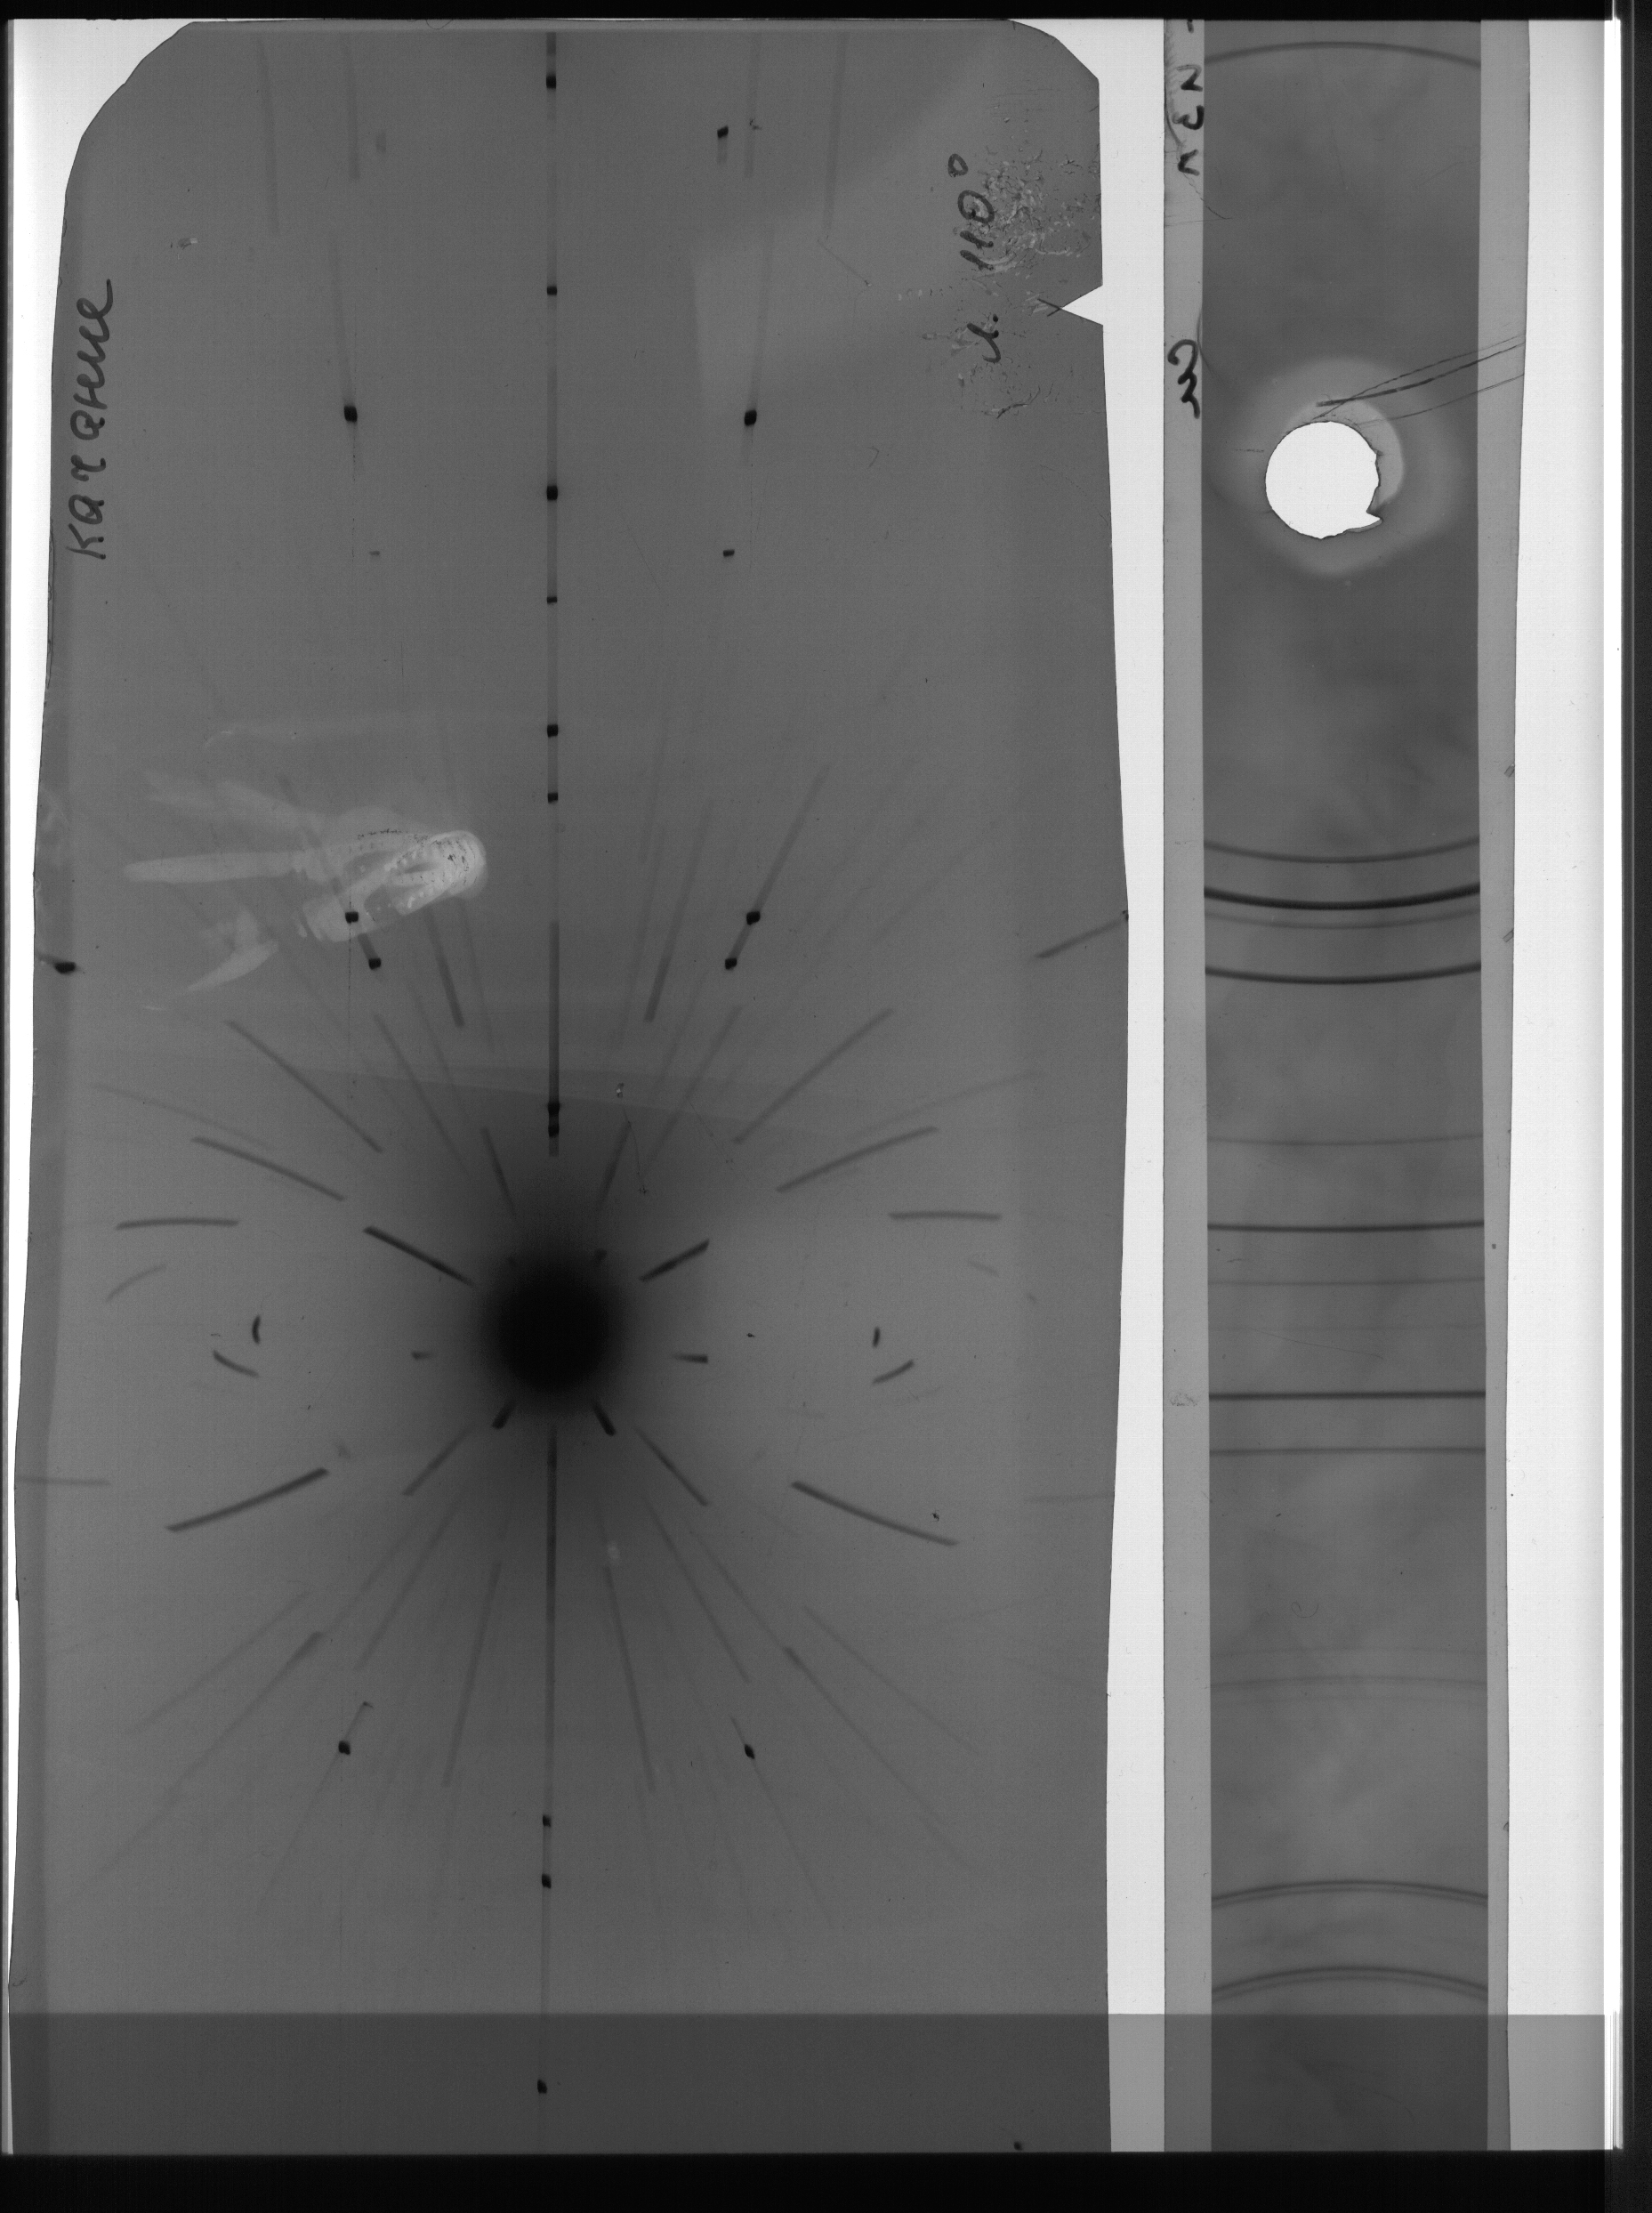
\includegraphics[width=0.7\linewidth, angle=-90]{3a.jpg}
	\caption{Исходная дебаеграмма}
	\label{fig:debae}
\end{figure}

Чтобы ее проанализировать, было измерено расстояние от линий, симметричных относительно отверстия (в правом верхнем углу), до центра отверстия, которое было принято началом отсчета. Результаты всех измерений, а также дальнейших промежуточных и финальных вычислений, приведены в сводной таблице.

С учетом используемой нами техники (камера РКУ-114), а также выбранного нами начала отсчета, измеренное нами расстояние до линии, выраженное в мм, соответствует величине угла $2 \theta$, выраженному в градусах. Это позволяет нам заполнить колонки со значением угла $\theta$, его синусам, а также квадратом его синуса.

Наличие линий с очень низкой интенсивностью наводят на мысль, что в дебаеграмме могут присутствовать $\beta$-линии. Согласно формуле (1.2)~\cite{Practicum}, <<для интенсивной, предположительно, $\alpha$-, линии с известным дифракционным углом $\theta_1$, можно определить ожидаемое расположение $\theta_2$ более слабой соответствующей $\beta$-линии, если использовать соотношение>>:

\begin{equation}
	\sin\theta_1 = f \cdot \sin\theta_2
\end{equation}

Здесь $f$ --- соотношение длин волн $\lambda(\beta) / \lambda(\alpha)$ для анода, с помощью которого проводится измерение. Согласно поступившим нам для обработки данным, при проведении эксперимента использовался медный анод, т.е. $\lambda(\alpha) = \lambda(\alpha_\text{ср}) \approx 1.54178$~\AA, а $\lambda(\beta) \approx 1.39217$~\AA, откуда получаем $f\approx 1.1075$. С учетом этого, заполним колонки $\sin\theta_\beta$ у $\alpha$-линий, у которых предполагаем наличие $\beta$-линии, а также колонку с типом линии.

Таким образом, для предполагаемых $\alpha$-линий, имеющих $\beta$-линии, проверим, совпадет ли теоретическое положение $\beta$-линии с тем, которое мы видим в реальности. Если да, то мы верно определили тип и принадлежность $\beta$-линии.

Отдельно отметим, что при достижении достаточно больших углов $\theta$, на дебаеграмме появляются расщепления дублетов. Для линий, составляющих дублет, в таблице будем использовать соответственно обозначения $\alpha_1$ и $\alpha_2$.

Для расчета межплоскостного расстояния $d$ воспользуемся условием Вульфа-Брэгга (формула (1.1) \cite{Practicum}):

\begin{equation}
	2 d \sin\theta = \lambda \qrq d = \frac{\lambda}{2 \sin \theta}
\end{equation}

Здесь $\lambda$ --- значение длины волны, которое для $\alpha$-линии, соответственно, берем равным $\lambda(\alpha_\text{ср}) \approx 1.54178$~\AA, а для $\beta$-линии равным $\lambda(\beta) \approx 1.39217$~\AA. Для линий, составляющих дублет, используем соответственно $\lambda(\alpha_1) \approx 1.54051$~\AA~и $\lambda(\alpha_2) \approx 1.54433$~\AA.

На следующем этапе определим индексы линий, предполагая кубическую структуру образца. Для этого согласно методике, изложенной в \cite{Practicum}, первой линии мы припишем индексы (111). В таком случае, для всех последующих линий, определение суммы квадратов индексов производится по формуле:

\begin{equation}
	\frac{\sin^2\theta_2}{\sin^2\theta_1} = \frac{h_2^2 + k_2^2 + l_2^2}{h_1^2 + k_1^2 + l_1^2}
	\label{eq:theta}
\end{equation}

Которая в свою очередь получается из формулы, связывающей межплоскостное ра
сстояние $d$ и индексы линий $h, k, l$ для кубической решетки:

\begin{equation}
	\frac{1}{d^2} = \frac{h^2 + k^2 + l^2}{a^2}
\end{equation}

Таким образом, на основании формулы (\ref{eq:theta}), заполним колонку таблицы с суммой квадратов индексов, на основании которой уже заполним колонку с самими индексами в предположении, что $h \ge k \ge l$.


\begin{table}[H]
	\centering
	\begin{tabular}{|c|c|c|c|c|c|c|c|c|c|c|c|c|}
		\hline
		$N$ & $I_\text{отн}$ & $l$, мм & $\theta$ & $\sin\theta$ & $\sin\theta_\beta$ & $\sin^2\theta$ & $\sin^2\theta (111) $ & $\sum\limits_i h_i^2$ & $d$, \AA & $hkl$ & $\alpha$/$\beta$ & $a$, \AA \\
		\hline
		1 & 6 & 39 & 19.5 & 0.3338 & & 0.1114 & 0.0371 & 3 & 2.3093 & 111 & $\alpha$ &   \\
		\hline
		2 & 10 & 43.5 & 21.75 & 0.3705 & & 0.1373 &  & 4 & 2.0803 & 200 & $\alpha$ &   \\
		\hline
		3 & 2 & 45 & 22.5 & 0.3826 & & 0.1464 &  & 4 & 1.8189 & 200 & $\beta$ &   \\
		\hline
		4 & 9 & 50.3 & 25.15 & 0.4249 & 0.3837 & 0.1806 &  & 5 & 1.8139 & 210 & $\alpha$ &   \\
		\hline
		5 & 1 & 65.6 & 32.8 & 0.5417 & & 0.2934 &  & 8 & 1.2849 & 220 & $\beta$ &   \\
		\hline
		6 & 8 & 73.8 & 36.9 & 0.6004 & 0.5743 & 0.3605 &  & 10 & 1.2839 & 310 & $\alpha$ &   \\
		\hline
		7 & 1 & 79 & 39.5 & 0.6360 & & 0.4045 &  & 11 & 1.0943 & 311 & $\beta$ &   \\
		\hline
		8 & 0.5 & 83.2 & 41.6 & 0.6639 & & 0.4407 &  & 12 & 1.0484 & 222 & $\beta$ &   \\
		\hline
		9 & 8 & 89.5 & 44.75 & 0.7040 & 0.6356 & 0.4956 &  & 13 & 1.0949 & 320 & $\alpha$ &   \\
		\hline
		10 & 3 & 95 & 47.5 & 0.7372 & 0.6657 & 0.5435 &  & 14 & 1.0455 & 321 & $\alpha$ &   \\
		\hline
		11 & 0.5 & 113.7 & 56.85 & 0.8372 & & 0.7009 &  & 19 & 0.8314 & 331 & $\beta$ &   \\
		\hline
		12 & 1 & 116.7 & 58.35 & 0.8512 & & 0.7246 &  & 20 & 0.8177 & 422 & $\beta$ &   \\
		\hline
		13 & 0.5 & 118.5 & 59.25 & 0.8594 & & 0.7385 &  & 20 & 0.8099 & 422 & $\beta$ &   \\
		\hline
		14 & 6 & 136 & 68 & 0.9271 & 0.8371 & 0.8596 &   & 22 & 0.8307 & 332 & $\alpha_1$ & 15.1830  \\
		\hline
		15 & 5 & 136.7 & 68.35 & 0.9294 &  & 0.8638 &  & 22 & 0.8307 & 332 & $\alpha_2$ & 15.1840  \\
		\hline
		16 & 6 & 144 & 72 & 0.9510 & 0.8587 & 0.9045 &  & 24 & 0.8098 & 422 & $\alpha_1$ & 14.4304 \\
		\hline
		17 & 5 & 145 & 72.5 & 0.9537 & 0.8611 & 0.9095 &  & 24 & 0.8096 & 422 & $\alpha_2$ & 14.4212  \\
		\hline
	\end{tabular}
\end{table}


\newpage


\begin{thebibliography}{1}
	\bibitem{Practicum}
	Рентгендифракционные методы изучения структуры монокристаллов, поликристаллических и аморфных материалов
\end{thebibliography}




\end{document}